\documentclass{project}
\usepackage[pdfauthor={C. P. Marriott},pdftitle={Software Engineering Group Project, Project Plan},pdftex]{hyperref}
\usepackage[pdftex]{graphicx}
\usepackage{pdfpages}
\hypersetup{colorlinks=false,pdfborder={0 0 0}}
\begin{document}
\title{Software Development Life cycle}
\subtitle{End of project report}
\author{Tom Reed, Matt Whitmore, Dave Clark, Silhab Csoma, Mike Steel, Chris 'Tux' Lloyd, Aleksandra Badyda, Samuel Jackson, Chris Marriott}
\shorttitle{End report}
\version{1}
\status{draft}
\date{2013-02-07}
\configref{SE.17.DS.01}
\maketitle
\tableofcontents
\newpage

\addcontentsline{toc}{section}{0.1   \ Project Plan}
\includepdf[pages=3-25]{./ProjectPlan/projectplan.pdf}

\addcontentsline{toc}{section}{0.2 \ Test Report}
\includepdf[pages=3-14]{./TestPlan/finaltestplan.pdf}

\addcontentsline{toc}{section}{0.3   \ Design Section}
\includepdf[pages=4-22]{./DesignPlan/DesignDocument.pdf}

\addcontentsline{toc}{section}{0.4 \ Maintenance Manual}
\includepdf[pages=3-12]{./projectMaintenanaceManual/maintenance.pdf}

\section{Reflective Reports}
\subsection{Aleksandra Badyda}
The project Monster Mash, while being largely enjoyable to work on, has under-
gone many changes since the beginning. This, together with the fact that the
information flow from Bernie to various groups was less than ideal, has caused
quite a bit of chaos, and forced us into rewriting most of the back-end code
during a Tuesday afternoon and the week that followed.
\\\\
My task was to be in charge of version control (via using GitHub as our platform
of choice) as well as writing up the HTML and CSS for the front-end of the
application. I’ve volunteered for both tasks, mainly due to my previous work
experience as a part of a small web developer group. The main task that I had
to deal with was teaching my group mates the basics of using git and later on
fixing up various mistakes or just maintaining some sort of order in the project
repository.
\\\\
Work with my group members has been a pleasure, despite one of two moments
when the pressure has gotten the better of me. Overall, given our circumstances
and the amount of work that we have all put into the project, I feel that it was
a very worthwhile activity and certainly a pleasant one, despite all the stress
in the testing and implementation week. We’ve been lucky enough making sure
that everyone worked at least a little and avoided any sort of a major crisis.

\subsection{Dave Clark}
My initial thoughts when we were first told we had to develop a project within a group of 9 people; it seemed rather a daunting task, as I didn’t know who I would be working with or if the group would get along as a whole. The project being a monster mash game seemed interesting enough and I thought it seemed a good project to work on. I also hoped that there would be people in my group who would be keen and eager to get started on the project. 
\\\\
My first memory of the project was meeting up in AberVaults to meet my fellow group members as arranged by a Facebook group set up to announce meetings and general news to the group as most people have Facebook. Here we discussed ideas, designs and functionality; we also used the time to get to know each other.
\\\\
The best thing about the project I thought was meeting new people I might not have talked to otherwise and improving relations with fellow students who do the same module. It also made you think about working more as a bigger group and how you had to co-operate together to get tasks done.
\\\\
My final impression of the project was; I felt that we had done a good job at implementing the game, as we only had 2 functional requirements missing. We worked well as a group and always seemed to get on with each other.
\\\\
In summary I thought it was a worth-while thing to do. I learnt a lot about how to work as part of a group of people to develop a game. This was a change to working on my own or in a smaller group. It gave me an insight into how you needed to do things differently when working as a group and how it helped to have such software such as version control and control forms to keep on top of things and to help manage a project more successfully.

\subsection{Christopher Marriott}
The task that we were set for this assignment was to create an interactive monster fighting/breeding selling game that could interact with other servers over the web. At the start of this project we all met up for the first time to meet our other team members and get to know them. Upon first meeting a few roles were set out, the first role that was assigned was my own, this was for me to be project manager. The reason being was I came with my laptop and a pen and paper to take notes. We also discussed peoples strengths and weaknesses in the group. I was very fourtunate to have a rather large group in which everyone had a different part they would be happy to work on.
\\\\
At this first meeting we discussed things like what it would look like and a few other minor details. If I had the chance one thing I would have done then is steer the conversation more towards the technical aspect of the system first. At the end of the meeting we decided to meet up more regularly and set a more regular date od weekly on Thursdays. At the next couple of meetings more detailed roles were decided for people and work began on the system and documentation.
\\\\
Next the we worked on creating the project plan and risk assesment, designing the interface and the database design and handling. This seemed to go rather well and we managed to get a decent project plan in on time. Some of the system had started to come together by this time. The whole team seemed to be working well together with people exchanging ideas and with no one person trying to tackle it all themselves.
\\\\
As the weeks went on we worked on creating all the documents required, with team members learning \LaTeX to aid in the document standards and GIT to keep everything backed up and safe. The systems parts were coming along nicely at this point. Then the christmas holidays came and work slowed down a little. As Project leader I felt I should have been more on top of this and keep everyone more informed and provided more tasks. When we came back after the holidays we were all aware that there was a lot of work that had to be done.
\\\\
As the deadline approached so did 'Intergration and Testing week'. This was where the team really pulled together to produce some amazing work. Major credit should got to both Samuel Jackson and Chris 'Tux' Lloyd who work amazingly as a team and got the system working up to the point its currently at. Other team members performed well during this time such as Tom Reed who kept documenters up to date with tasks and allowed the programmers to continue on with their work and reported issues/bugs to them as and when needed.
\\\\
I feel this project went well and everyone suited the roles that they were assigned. However, I believe I could have performed better as project manager by keeping more on track than I did and on several occasions I had to ask for help from Samuel Jackson who helped me out as deputy project manager. The overall result of the system is brilliant with excelent documentation. I could not have asked for a better more well rounded group.

\subsection{Samuel Jackson}
My role in the group project was to be one of the main programmers for the front end of the site and to aid with the general design of the system. While the finished system which we produced managed to meet most of the requirements outlined in the brief, I feel that there were a lot of things that hindered the progress and development of the project more than there could of been.
\\\\
On the whole, I felt that the majority of the early part of the project went reasonably well. Our team managed to schedule and attend regular meetings and could set targets and activities to each of the team members and generally kept to the deadlines set by the project manager. I also feel that people were adequately assigned to their roles according to their programming/design experience and individual preferences.
\\\\
However, I feel one of the major flaws with the project was the failure to fully analyse the implications of the design we produced. This lead to the design team (myself included) designing a system that could not work in the way intended. This was largely because of concurrency issues when multiple users are logged into the system.
\\\\
Subsequently, much of the back end of the system needed redesigning on the fly during the early stages of implementation and testing week. This later caused knock on delays with implementing some functional elements of the system (e.g. ageing and server-to-server communication) as well as delaying the start of the testing phase.
\\\\
This coupled with the added hindrance of frequent university network outages meant that we had to make strategic practical decisions in order to get as many of the functional requirements up and running by the Friday deadline. This included actively deciding to drop some of the more subtle functional requirements in order to concentrate on the more important elements of the system (i.e server-to-server communication). If this were a real software development project, I believe that the user would either of been force to accept a lower quality of product or grant the team an extension of another couple of days.
\\\\
I would like to outline at this point that if it were not for the network outages I have full confidence in that fact that our team would have been able to get at least one of the missed requirements serviceable by the deadline and quite possibly both of them.
\\\\
Turning to the more positive elements of the project, the logical data structures and algorithms (such as those used for battling and breeding) which were developed in isolation from the rest of the system and integrated during coding week work straight out of the box. When it came to there integration, all that was needed was for Monster objects to be passed in and the pre-written code did the rest. This meant that more development time could be devoted to other issues with the system.
\\\\
A key factor in the success of the this project was largely down to the rigour and efficiency of the testing team. Once we had the system to a working but highly buggy stage, the testing team was set loose on the project and ran through all the tests in our test plan and later also using the user acceptance tests emailed out by Bernie, as well as any other creative tests they could think of. I feel that a large part of any successes we made is a down to them.
\\\\
As we were on such a tight schedule, it was imperative that feedback from the testers reached the programmers as quickly and efficiently as possible. To do this, whenever a bug was found with the system, it was written on paper under the name of the developer responsible for the code that caused it. Each developer then worked through each of the bugs while the testing was still running and attempted to fix each issue. The project would then be redeployed and testing would begin again from scratch. Any new or continuing issues would then be identified and reported. 
\\\\
This cycle continued until all implemented functional requirements passed. This system worked well because it allowed all members (QA's and developers) to be active on the project at the same time, meaning it became very efficient to weed out bugs.
\\\\
Another technique that was applied to the project that I felt worked quite well was the use of a pair programming technique between myself and the lead server side developer. Because of the issues already outlined in this document, we were often forced to work long hours implementing and integrating the client side and server side of the system. 
\\\\
By working closely together, carefully discussing and occasionally editing each other's code, it allowed use to reduce difficulties getting the two components of the system to talk to each other. It also allowed us to brain storm effective solutions to problems encountered along the way and let us double check what we had each written. This was especially useful when writing SQL queries and JSON strings while sleep deprived where spelling and formatting are paramount.
\\\\
In conclusion, I feel that the implementation of this project could have gone smoother and some aspects could have been better outlined/developed/analysed, but in general I am happy with the outcome. Furthermore, I would like to outline once again how despite the setbacks and design obstacles our team encountered with the project, I feel that all team members pulled there weight and that producing a system to the level delivered would have been impossible without the effort exhibited by every member group 17.

\subsection{Silhab Csoma}
When we first started this project, things looked optimistic, we would have a lot of meetings and started working on the initial design early. Everyone was friendly and we delivered most of the documentation in time with only minor issues. 
\\\\
Then, coding week came, and things got a lot more chaotic both for us and all of the other groups as well. Suddenly, the requirements for the project started changing, causing most of the coding we have done up until that point to need rewriting. The campus network would do the impossible and become subject to a major hardware failure, hindering our work and causing us to lose some of our progress. Despite all difficulties, everyone tried their best to deliver as much work as possible and we managed to deliver all but 2 of the requirements in the specification. We even did some bonus features like a help page, a feature to rename monsters and added some detail into the notifications.
\\\\
In this project, I was a programmer for the straight Java side of the code, I also wrote the testing and some of the documentation related to my work.  I helped with the server side as well, mostly with logic problems and some Java functionality. While the communication between Sam and Tux for JavaScript and server side Java was strong, the Java side could have been better. I feel like we could have avoided some of the rewriting of the code if I had received more specifics about how they wanted the two parts of the program to come together.
\\\\
Still, I learned a lot about working together as a group as well as how to create a functional web based application. We fulfilled most of the requirements, if it wasn’t for the complications during coding week, we could have certainly done even more.

\subsection{Tom Reed}
Role: QA Manager\\
For this assignment we where put into groups and assigned the task of creating an online
game based around users owning monsters and being able to add friends in order to
battle their monsters or breed with their monsters. During the assignment I was given the
role of the QA manager. This role needed me to manage various people and ensure that
the project met various standards that would need to be set in order to produce the best
possible system.
\\\\
Positives\\
During this assignment I felt that I worked well within the group, there was no conflict
within the group and as a whole we all got on well with each other. I felt that because of
this it was fairly easy to manage people within the group which is something I felt I did well.
I also feel that I distributed various tasks to members of the group fairly and efficiently by
giving the most competent person in a given area the task that fits their skill set the best.
This was something that I tried to do for every task to ensure that the best possible
outcome was produced. I also feel that I was able to complete tasks that I had been given
on time and to the best standard possible.
\\\\
Negatives\\
Allow this whole assignment was mainly positive I have some negative points. When I first
started as QA manager I did not have much knowledge about QA. This meant that I had to
do a lot of research and as questions os that I could fully understand what was needed of
me for this task. I also feel that my lack of programming knowledge hindered me during
this task as I did not fully understand the back end Java of the system that was developed
this again meant that I had to ask a lot of questions and ask of explanations of that was
going on.
\\\\
What I would have done differently\\
If I where to do this task again I would concentrate more of overall time management for
the group. Although we met every deadline I still feel that we would have managed our
time better and been more efficient. I also feel that I could have been a bit tougher and
assertive as a manager, more demanding with deadlines .etc. I also thin that I could have
spent more time planning and researching the standards and other plans that where set
out in order to use our time as efficiently as possible. If I where to do this task again I
would defiantly prefer to do a more hands on role as appose to a more overseeing role
that I had in this instance. Although I did work hard at this role and appreciate that
experience that I have gained from it I feel that a hands on role is more enjoyable and
rewarding.
\\\\
Summary\\
Overall I feel that I preformed well in this task. I managed people well and completed task
assigned to me on time. Although there where some areas that I struggled with during this
project I feel that I over came them. I think that I have learnt a lot from this assignment,working with a medium sized team, managing people, time management for a project,
working with new people. Although I would have preferred to have done a more hands on
role I did enjoy my role as QA manager and worked hard to understand the role and also
to produce the best result.
\\\\

\subsection{Chris 'Tux' Lloyd}
On Monday evening of coding week, the coders were made aware that the requirements document had been changed. Breed and buy were no longer operating on a request accept/deny system, but instead an offer system. Due to this it meant that extra fields needed to be added to the monster table in the database. Because of the alteration to that database, it meant that all code relevant to the monsters was now invalid. This meant we could no long do anything as the backend would crash on login due to the fetching of monsters, couldn’t even create a new account, as a monster was generated and added to that new account. All this needed to be fixed before I could start to rewrite the breeding and buying. I feel that someone should have really informed the coders before coding week.
\\\\
Sam and I worked well as team and paired programed for the bug fixing as I handled all the back end and Sam did the java script allowing both of us to get short breaks while still thinking and working on solutions to issues. The documenters also proved to be invaluable to the coders as they would run a full requirements check and the let us know about the issues that came up and Sam and I would work though them. Sam was a big help in keeping me from breaking down and focus on the task at hand.
\\\\
I had to rewrite some of silhabs classes so that it worked with the rest of the code. More effort should have been put into getting those 2 parts of code to work rather than me doing a rewrite. Silhab did make good use of time and write the joint test in a black box environment that helped with the testing process.
\\\\
The IS server outages caused mayor disruptions to our work flow as we were not able to make commits to git or deploy to my tomcat server. Also not having internet at my house meant that Sam and I spent hours waiting for the connection to return to commit our changes so our latest work would not be lost. Also the M-drive outages were problematic as that is where my eclipse workspace was pointed, this was an issue as my pc was the one that Sam and I were programing on.
\\\\

\subsection{Mike Steel}
From the outset our project team has been clearly organised into one group who are more comfortable with code and one group who are more comfortable with documentation, this has been helpful during each stage of development, as it was defined early on who would be best at each task. By giving each documenter a specific part of the code to document it allowed them to get to know the person working on that part of the code, as well as get to grips with how that part of the program would function and allow for documentation. As you can probably tell from what I have mentioned so far, I was a member of the documenting team, and had little part in the actual coding of the program, however, even though the documenters and the coders worked relatively seperately on the different parts of the project, when we needed to consult with each other over designs and the like we worked together well, and as a whole the group itself worked together well as a single unit completing each necessary part of the project.
\\\\
By the time it came to implementation and testing week the group were used to working together enough that the final implementation of the project and especially the testing worked out very well. Most people turned up when required so that documentation was completed between testing phases, and the optimum amount of work was done for the time that we had. If there had not been the network problems and last minute project specification changes then we would have most certainly finished all functional requirements of the project, and it is a shame that those problems that we encountered were out of our control. Overall, the final outcome of the project is something that I am very happy with, and would work with the same group again any time. We all did what needed to be done, and helped each other out as well as included everyone in decision making.
\\\\
I have enjoyed this project very much, and even though at times the work load has been more than I was expecting I know that some group members have worked on this project for far longer and harder than I would ever be able to make myself do, and I am truly impressed by some of the levels of work that some group members have put into this project. The experience has certainly prepared me for future group work, both in future university projects and in the world of work. This project has made me a more able group member, and has allowed me to experience every stage of an industry-worthy project. Therefore, I am now a more competant and experienced worker, and ready to do more work within groups in the future.



\section{Management Summary}
This project has managed to achieve 25/27 of the functional requirements it was aiming to complete. See (cite requirements doc) for list of functional requirements. The only two that were not managed to be completed on time were, monster aging and server to server. The mosters ageing requirement, although not implemented, there was a formula that we had that worked. Given a bit longer on the project I believe we could have got the monster ageing working. The server to server side however was a bit further off. Silhab Csoma had a look at the server to server but due to the change in requirements and internet down time there was not time to implement server to server.
\\
All the documents have been worked on thoroughly and I feel that they are up to a more than reasonable standard.
\\
\\
A few difficulties got in our way during the development of the system. One of these issuses was the change of requirements. Originally it was specified that the monster battle and breed would be offered up or requested but as the deadline approached the functional requirements were changed to specify that breed and battle requests had to be offered. This meant that part of the system had to be redesigned which took time off working on bugs and other functional requirements. 
\\
\\
Another major issue that arose was that there was internet downtime in the week before the deadline. This caused several issues, the first of which was the inability to test the system properly. This lead to work on the system being slowed down and thus resulted in a less complete system. It also meant more two of the coders(Sam Jackson and Chris 'Tux Lloyd) had to put in more hours to complete what was necessary to get a functional and bug free program. 
The second issue the internet downtime caused was a loss of work as when uploading the latest copy to git there was an error in doing so. We then tried to access the project which was stored on the M: drive however, this was unaccessable. We decided to leave the university grounds and head down into town to find somewhere with a working internet connection. Here the two coders managed to get access to the temporarily back up internet and M: drive and obtain a copy of the latest code. From here it was then uploaded to GitHub with an issue that meant the latest CSS code would be Lost. This meant Aleksandra Badya had to put more work into finishing of the design of the system.  
\\
\\
The team preformed outstandingly overall. However special credit has to go to Chris 'Tux' Lloyd and Samuel Jackson as they worked perfectly as a team. Between them they managed to sort out a large quantity of the bugs and get a large chuck of the system operational. The rest of the team fulfilled there roles and more, they managed to do what was asked of them and more. 

\section{Historical account of project}
The main events of this project were as follows;
The first main event that happened was the meeting of the group. This is classed as a main event as we did not all know each other so we decided to meet up and get to know one another so we would find it easier to work with each other. This proved a good idea and thankfully every team member seemed to get on well with each other. We also assigned tentative roles to team members.
\\
Next we started work on creating the system and project plan document. During this document creation we had weekly meetings and regular reviews of the document. The system was also starting to take shape at this time with parts started to be developed. 
\\
After the project plan document we moved onto the test specification document and designing the web interface. Again with this document we also had weekly meetings and reviews of the documents being produced. As well at this point in the project team members were getting more familiar with using \LaTeX to standardise documents and github for version control. System continued to develop at this point.
\\
Work then began on the design specification document for the system and getting a prototype ready for demonstration. The whole group worked briliantly on documenting, testing and implementing all aspects of the system. After this we worked on improving the documents and the system up to a standard that would be ready to hand in.
\\
The final stage of this project was 'testing and implementation week' where the project was developed into the best state it could be. Here Samuel Jackson and Chris 'Tux' Lloyd managed to get more or less the whole system working even after internet down time cause issues with the project as well as a change of functional requirement. The documentors helped by testing the system and reporting any issues/bug so they could be fixed. Then the final document was produced which is a combined working of all the documents that have been worked on.
\\
The team worked very well with each other communicating when needed and completing tasks set for them. 

\section{Final State of project}
The final state of the project is that 25/27 of the functional requirements were fulfilled. The only two requirements that were not fulfilled were the monsters ability to age and the ability to connect server to server. 

This should give a summary of which parts of the project are perceived as correct and
which are not. It is as well to be as accurate as possible here - more marks will be deducted for problems that are
not declared but are detected by the markers than for problems that are declared in the final report. As well as
missing or erroneous features in the software, known problems with documents should be included here.

\section{Performance of each team member}
\subsection{Tom Reed}
Tom's duties as Q.A. Manager were to manage other documentors and delegate documenting tasks where he felt appropriate. He preformed brilliantly especially as the deadline approaced, he assigned tasks well and made sure they were completed. He also kept Christopher Marriott(Project Manager) up to date on goings and asked for more work when finished allcurrent work. He was an worked brilliantly in the team and helped the dynamic of the group flow.  

\subsection{Chris 'Tux' Lloyd}
Tux preformed outstandingly. His time and effort put into the code was brilliant and he worked well with the rest of the team. He informed people of changes and explained things clearly. He worked especially well in tandem with Samuel Jackson. He put countless hours of work into the project and helped solved numerous bugs. Tux worked on the server side of things, getting the connectivity working with Samuel Jackson and Silhab Csoma side of code.

\subsection{Samuel Jackson}
Sam's preformance was outstanding. Not only was he vital in the functionalality of the overall system but on occasion preformed as a brilliant project leader when Christopher Marriott was away. His main role was to work on Javascript for the system. He helped get the system up and running and helped keep the team on track with their roles. He also put in a large amount of time into the project during coding week.

\subsection{Silhab Csoma}
Silhab worked on data structions and worked on algorithms this was essential to the working of the system. Without these in place there would be no way of storing monster and user info. Also the battle requirement would not be completed if it was not for the algorithm designed. Her testing on parts of the system helped other team members progress in their work. She worked well in a team and completed all tasks set. 

\subsection{Alexsandra Badya}
Alex worked very well in the team. She provided vital support to the team with git support, whenever there was and query or issue she was able to help resolve the problem. Here main role however was the creation of HTML and CSS for the system and in this role she performed very well. She also worked well as deputy Q.A. manager when Tom Reed was away. The team were kept up to date with duties they had to complete. She performed very well on the whole project.

\subsection{Dave Clark}
Dave was a very good documentor in all areas. He mostly focused on Tux's server side documentation however he also work on other documentation. He also helped find bugs with in the system and inform people of what they were. Other areas he worked on were the database diagram, methodology and reviewing functionality. He also did the minutes for several of the team meetings.

\subsection{Mike Steel}
Mikes main duty was to document Silhab's work. He performed well within the team and helped in other areas. He helped out on the testing side of the system and fixing the \LaTeX  documents. He also produced the risk assessment and designed the monster mash logo that we use on the main system webpage. He helped update documents and fix any mistakes with them.

\subsection{Matt Whitmore}
Matt's job was to document and test Alex's HTML and CSS. He completed all tasks on time and worked well with the team. He also helped out on the testing of the system and found some bugs of which he informed the appropriate people. 

\subsection{Christopher Marriott}
Chris' main role was project manager. As project manager it was Chris' duty to assign tasks to other team members, review documents and check that people are completing their tasks. He communicated to the group regularly and organised meetings, he also on occasion took the minutes. He also helped out on the creation of documents and bug testing. He also got people to start using \LaTeX to help standardise documents.

\section{Critical evaluation of the team and project}
\subsection{Team performance}
The teams performance was brilliant. A few team members also went above and beyond the call of duty to get the system more or less fully functional. Everyone knew their role and were happy with the tasks they were set. If anyone had a problem they spoke to the appropriate person and got it resolved reasonably quickly. Everyone did their roles excelently and fulfilled all that was required and more. Each member of the team communicated clearly with other team members and kept up to date with what had been done and what had not. Each team member was kept up to date and informed of new tasks via a facebook page and a gannt chart. Everyone seemed happy with this approach and there was no major disruptions from within the group.

\subsection{Improvements}
The project could have been improved in a few ways. The first way would have been to assign Samuel Jackson as the project manager as he was more knowledgeable in the system and would therefore been able to assign more details tasks. The second would have been for Christopher Marriott(Team leader) to have informed the team of new tasks that needed doing and keep up to date with where team members were at with their current task.

\subsection{Lessons learnt}
Some of the lessons that were learnt during this project were to make sure people understood their role more clearly. To plan the more important and required parts of the system before worrying about how it will look. How to code alongside others, how to manage time more appropriately and skills in being a leader.

\clearpage
\addcontentsline{toc}{section}{REFERENCES}
\begin{thebibliography}{5}
\bibitem{} \emph{N/A}
\end{thebibliography}
\clearpage
\addcontentsline{toc}{section}{DOCUMENT HISTORY}
\section*{DOCUMENT HISTORY}
\begin{tabular}{|l | l | l | l | l |}
\hline
Version & CCF No. & Date & Changes made to Document & Changed by \\
\hline
1.0 & N/A & 2013-01-30 & Initial creation & cpm4 \\
\hline
\end{tabular}
\label{thelastpage}
\end{document}
